\documentclass[twocolumn]{article}
\usepackage{graphicx}
\usepackage{nameref}
\usepackage{amsmath}
\usepackage{amsfonts}
\usepackage{amssymb}
\usepackage{hyperref}
\usepackage{cleveref}
\usepackage{setspace}
\graphicspath{{./figures}}

\onehalfspacing

\begin{document}

\title{Disease Diagnosing via Machine Learning}
\author{
  Champagne, Matthew \\
  \texttt{matthew.champagne@stonybrook.edu}
  \and
  Khadka, Abiral \\
  \texttt{abiral.khadka@stonybrook.edu}
  \and
  Flores, Yasmin \\
  \texttt{yasmin.flores@stonybrook.edu}
}
\maketitle

\section{Abstract} 
Remote diagnosing and evaluation of several disease problems via the usage of telemedicine are vital in the monitoring and management of diseases such as: COPD, pneumonia, lung fibrosis, and arrhythmias. Traditional forms
of diagnosis and management of such disease problems have been shown to be reliable and useful,but lack the ability to provide a telemedicine option. The ability to provide a remote method to track and diagnose these diseases can open new possibilities to make the diagnosis of such diseases more accessible and require less visits to the doctor's office. In this paper, we provide a new perspective on this issue that is broken down into two phases, where phase one entails of creating and evaluating a machine learning model where we can load and preprocess data into a convenient data structure. While phase two involves finding capable hardware of running the model and creating an application that uses the model. Consequently, once combining these two phases with the dataset acquired from Jordan University of Science and Technology on sound data using a 3M Littman electronic stethoscope model containing 336 audio files that were annotated with the sound type and diagnosis and location on chest; our model accuracy was 85 percent and its precision was 86 percent. 


\section{Key Words} 
KEYWORDS: Machine Learning, Disease diagnosing, Electronic Stethoscope, Proactive Monitoring, Cardiovascular Disease Management, Telehealth 


\section{Introduction}
Proactive health focuses on preventing illness before it occurs through regular monitoring, early detection, and lifestyle adjustments. By addressing risk factors and making informed choices, proactive health promotes long-term well-being and reduces the likelihood of developing serious conditions. Similarly, monitoring diseases allows for the early detection of health problems, and offers the chance of early interventions that can prevent worse results. Thus why regular monitoring also aids in personalizing treatment plans, adjustment techniques as needed, and track progress over time. Consequently, improving the odds of a better outcome for patients with such diseases. A method that can be used in both proactive and regular monitoring of diseases is the usage of telehealth. Where telehealth refers to the ability to obtain remote healthcare services outside the doctors office. This approach not only decreases the frequent in-person visits to the doctors office but also improves patient engagement while potentially reducing the cost of visits. 

Comparatively, when diagnosing diseases, machine learning can be used to analyze large datasets of medical information, such as imaging, genetic data, or audio recordings, to identify patterns indicative of specific conditions. Where specified and tailored algorithms can be trained to recognize subtle differences in data that may enable faster and more accurate diagnoses. Afterward a model is trained, and these models can continuously be improved by learning from the new data, and enhancing their ability to detect diseases in diverse patient populations.

Where in this paper we used sound data collected using a 3M Littmann Electronic Stethoscope from Jordan University of Science and Technology, capturing recordings from various chest zones and transmitted via Bluetooth to a computer for processing with StethAssist Visualization software. Including 112 participants, and a wide range aged 12 to 90, with 35 healthy individuals and 77 with respiratory conditions such as asthma, COPD, and heart failure. Each participant contributed a 5 to 30-second audio recording, filtered in three modes to highlight different frequency ranges. 

Annotations on health conditions, sound types, and demographics make the dataset valuable for developing algorithms to diagnose pulmonary diseases.



\section{Background and Motivation} 
In this section, we first provide background knowledge on the importance of monitoring heart related problems and one of the most common standard methods used in heart disease evaluation via the usage of a stethoscope. We then introduce our new approach on a stethoscope design and its limitations of directly capturing a range of datasets.


\section{Importance of Monitoring Diseases} 
Monitoring diseases is essential for early detection, effective management and prevention of serious complications. According to the American Heart Association, regular monitoring for heart disease, assists in identifying risk factors such as:‘diet quality, physical activity, smoking, body mass index, blood pressure, total cholesterol, blood glucose and sleep quality’ [X]. In other words, regular monitoring not only allows the doctors to treat the patients’ health, but also make the necessary adjustments to optimize the treatment plan by considering several risk factors and improve long-term results. Ultimately, constant monitoring of diseases  can be viewed as a proactive method in lowering problems while also serving as an essential method to continuously better diagnose patients' who already have existing diseases. 


\section{Traditional Stethoscopes} 
One of the main instruments in diagnosing and monitoring a well known disease such as:heart related problems is a stethoscope as seen in figure 1. This medical tool is composed of three parts: a chestpiece, tubing and a set of earpieces. It then functions by amplifying internal sounds from the body through two important elements: vibrations and sound waves [2]. It works when the chestpiece/diaphragm is placed on the patient’s chest, where the heartbeat creates soundwaves that makes the chestpiece to vibrate. Where afterwards these vibrations make its way through the tubing and into the earpieces. At this point the doctor can begin to interpret the heartbeat and sounds. As shown in figure 2, there are four common breathing sounds when using a stethoscope which all can be interpreted when diagnosing a disease.

 \section{Data Collected}  
The sound data was collected using a 3M Littmann Electronic Stethoscope model 3200, positioned on specific chest zones divided into upper, middle, and lower sections on both the left and right sides, including anterior and posterior locations. The stethoscope transmitted sound data to a computer via Bluetooth, and the 3M Littmann  StethAssist Visualization software was used to extract recordings in .WAV format. The recordings were filtered through three modes (Bell, Diaphragm, and Extended) to emphasize different frequency ranges and highlight specific sound profiles.

The dataset contained 112 participants aged 12 to 90 years including 43 females and 69 males. Among these, 35 were healthy, while 77 had respiratory conditions such as asthma (32), pneumonia (5), COPD (9), bronchitis (3), heart failure (21), lung fibrosis (5), and pleural effusion (2). Each participant contributed a single recording lasting 5 to 30 seconds from specific chest zones. The data files included annotations detailing health conditions, sound types, chest zones, and demographic information, making these datasets a valuable resource for developing algorithms for detecting and diagnosing pulmonary diseases.


\section{Data Preprocessing} 
The preprocessing pipeline for the patient diagnosis model involves transforming raw audio data from WAV files into structured tensors suitable for machine learning algorithms. This process includes segmenting audio files, extracting key features such as spectrograms and chromograms, and assigning diagnostic labels to each sample, ensuring uniform preparation for training and evaluation. The first step in preprocessing is to split each audio file into 2.5-second segments (10,000 samples for a 4kHz sample rate) to maintain consistency in input length across all samples.

After segmentation, key audio features are extracted to capture both time-domain and frequency-domain information. A spectrogram is generated to represent the intensity of sound over time, where frequency is plotted against time with amplitude as the color intensity. In parallel, a chromogram is created to capture harmonic features that highlight breathing patterns. These features provide rich information about the underlying acoustic signals. Both features are resized to ensure compatibility in dimensions, and they are concatenated into a multi-channel tensor. The resulting tensor contains two channels: one for the spectrogram and another for the chromogram.

Label assignment is the final step in preprocessing. Each audio file is associated with a specific diagnosis based on the patient's ID or file naming conventions. Diagnoses such as COPD, Asthma, and URTI are mapped using a predefined dictionary, ensuring that each audio segment has a corresponding label. Additionally, metadata such as the stethoscope mode (bell, diaphragm, or extended) is derived from the file name or directory structure to enrich the dataset with contextual information.

\begin{figure}[h]
  \centering
  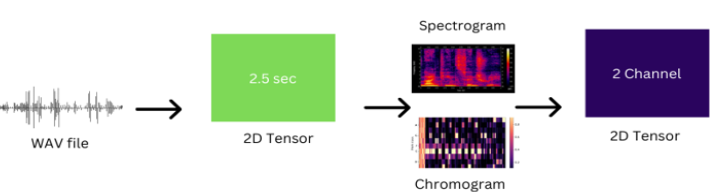
\includegraphics[width=0.5\textwidth]{Pre-Prrocessing}
  \caption{Overview of the Preprocessing for Audio Data}
  \label{fig:Pre-Prrocessing}
\end{figure}

\section{Convolutional Pipeline}
The convolutional pipeline begins by processing a 2-channel input tensor (e.g., spectrogram and chronogram) with dimensions \(2 \times 128 \times 64\). The first convolutional layer applies 24 filters of size \(5 \times 5\) with a stride of \(4 \times 2\) and no padding, reducing the spatial dimensions to \(24 \times 31 \times 30\). This layer is followed by batch normalization, which stabilizes feature maps, and a LeakyReLU activation with a slope of 0.01 to introduce non-linearity and mitigate the vanishing gradient problem. Next, a second convolutional layer applies 16 filters of size \(5 \times 5\) with a stride of \(1 \times 1\), further extracting complex features and producing an output size of \(16 \times 27 \times 26\). Similar to the first layer, batch normalization, and LeakyReLU activation is applied to ensure stable training and effective feature learning.

The pipeline then incorporates a max pooling layer with a kernel size of \(4 \times 2\) and stride \(4 \times 2\), down-sampling the feature maps to \(16 \times 6 \times 13\). A third convolutional layer applies 4 filters of size \(3 \times 3\) with a stride of \(1 \times 1\), extracting deeper hierarchical features and reducing the dimensions to \(4 \times 4 \times 11\). This is followed by batch normalization and LeakyReLU activation to maintain non-linearity and enhance learning. Finally, the output tensor is flattened into a 1D vector of size \(1 \times 176\), preparing it for downstream tasks such as classification or regression. This sequential architecture effectively reduces the input dimensions while capturing meaningful features for robust audio-based diagnostic predictions.

\begin{figure}[h]
  \centering
  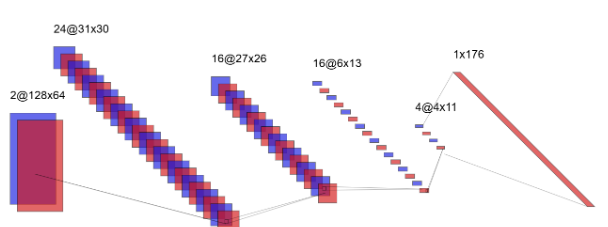
\includegraphics[width=0.5\textwidth]{Conv-Pipeline}
  \caption{Overview of the Convolutional pipeline}
  \label{fig:Conv-Pipeline}
\end{figure}

\section{Combined Pipeline}
The combined pipeline integrates scalar and multidimensional inputs, processes them through a series of fully connected layers, and outputs predictions using a softmax function. The design is structured to progressively reduce dimensions while maintaining robust feature representation through non-linear activation and normalization techniques.

The scalar pipeline starts with a single linear layer that transforms a scalar input to the desired scalar output size. A LeakyReLU activation with a slope of 0.01 is applied to introduce non-linearity, enabling the network to capture complex relationships in the scalar input.

The combined pipeline begins by accepting the concatenated input vector which merges outputs from earlier stages. The first fully connected layer reduces the input to 1024 dimensions, followed by batch normalization to stabilize the training process and LeakyReLU activation for non-linearity. Dropout with a rate of 0.5 is applied to prevent overfitting. This pattern is repeated across four subsequent layers, progressively reducing dimensions from 1024 to 512, 128, 64, and finally the size of 8. At each stage, batch normalization and LeakyReLU activation enhance feature extraction, while dropout ensures robust generalization.

The final layer applies a softmax activation, converting the output into probabilities over the target classes. This combined pipeline effectively integrates scalar and multidimensional data, utilizing deep learning techniques to achieve accurate and interpretable predictions.

\begin{figure}[h]
  \centering
  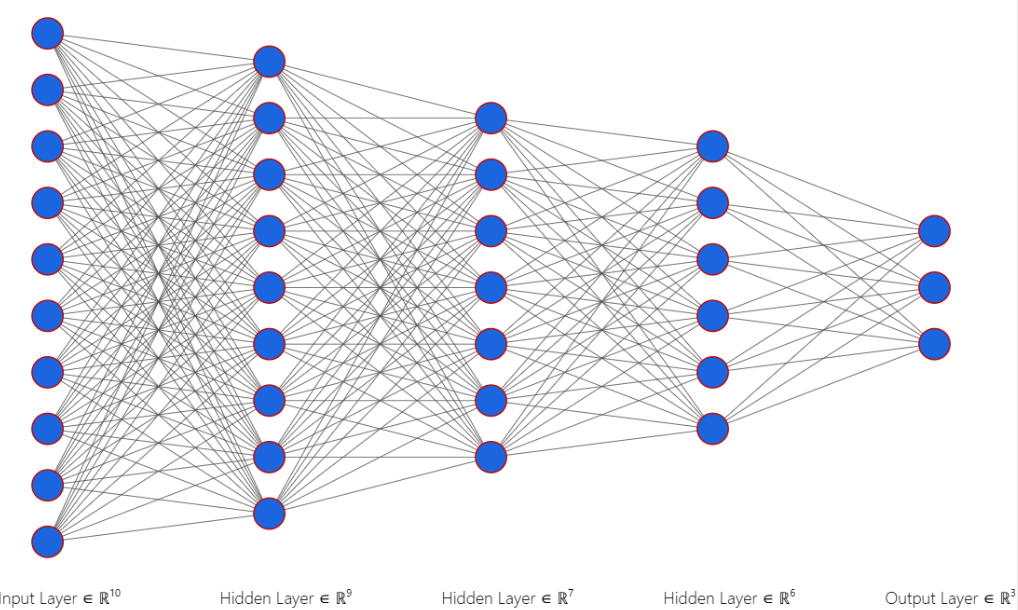
\includegraphics[width=0.5\textwidth]{Main Pipeline}
  \caption{Overview of the Combined pipeline}
  \label{fig:Main Pipeline}
\end{figure}

\section{Model Evaluation}
The model achieved an overall accuracy of \(88.81\%\), correctly classifying 365 out of 411 test samples. This high accuracy indicates the model's strong ability to generalize across diverse diagnostic categories. The weighted precision of \(88.81\%\) shows the model's effectiveness in minimizing false positives, ensuring the majority of predicted classes are correct. Similarly, the weighted recall of \(88.81\%\) highlights the model's ability to identify actual positive cases accurately, demonstrating excellent sensitivity. The F1-score of \(88.81\%\), a balanced measure of precision and recall, further emphasizes the model's robustness and consistency.

From the class-wise analysis, categories like Asthma and Bronchiectasis exhibit strong correct prediction counts, with Asthma achieving a precision of approximately \(87.96\%\) and Bronchiectasis achieving high performance in both total and correct predictions. This consistency across major classes underlines the model's reliability. Furthermore, even for less frequent classes like Lung Fibrosis and Pleural Effusion, the model maintains stable prediction patterns, showing its ability to handle class imbalances. These results confirm the model's readiness for real-world diagnostic applications, supported by its high overall performance across metrics.

\begin{figure}[h]
  \centering
  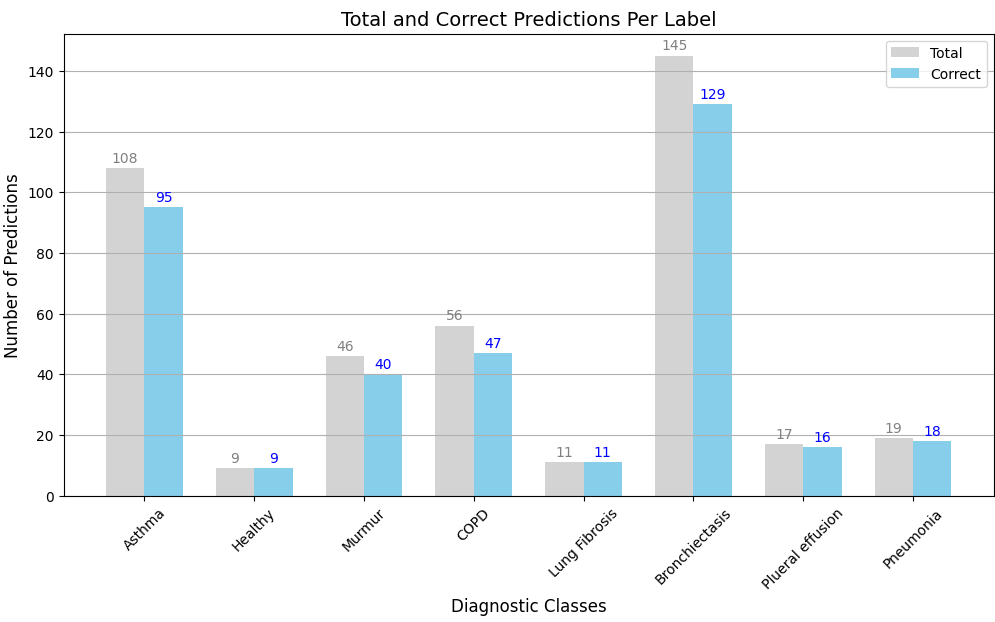
\includegraphics[width=0.5\textwidth]{Diagnostic}
  \caption{Overview of Model Accuracy}
  \label{fig:Diagnostic}
\end{figure}

\section{Application}
As a proof of concept we wanted to take the model we trained and deploy it into a useful independent mobile device. We wanted to do this to show that even on pedestrian hardware the model isn't to expensive to use.

\subsection{Hardware Design}
When considering what hardware to choose we wanted to minimize the cost as well as the development time.
These were our main priorities because we had no funding and a limited time budget.
This drove us to pick well supported hardware with open source hardware drivers. 
The Raspberry Pi fit this criteria perfectly along with the TFT-LCD, the USB audio interface, and the contact microphone (Links to the hardware selected can be found in the associted README).

 \begin{figure}[h]
  \centering
  \includegraphics[width=0.5\textwidth]{Compute_LCD}
  \caption{Diagnostic App User Interface}
  \label{fig:Compute_LCD}
\end{figure}

\begin{figure}[h]
  \centering
  \includegraphics[width=0.5\textwidth]{Audio_Interface}
  \caption{Diagnostic App User Interface}
  \label{fig:Compute_LCD}
\end{figure}

\subsection{Software Stack}
The software was developed in Python to maximize code reusability, particularly for preprocessing and cleaning tasks used during model training. 
Libraries such as Tkinter are utilized for creating a user-friendly graphical interface, while PyAudio and Librosa handle audio recording and processing tasks. 


As a consequence of the software being fully built in python the application is fully cross platform and can run on any desktop operating system. In order to get the application to boot directly from the Pi with no intervention in full screen mode we setup the application as a systemd service. 
The systemd service would simply launch a X11 server along with a window manager and the application. 
From the perspective of the application this enviroment is entirely equivalent to a linux desktop. This allowed the integrated touch screen to work with very minimal configuration because a driver already existed for it in the kernel that would treat as a X11 mouse.


\subsection{Functionality and User Interface}
The diagnostic application simplifies the diagnostic process for end-users. It operates as follows:  
1. The user presses a "Record" button, initiating a 10-second recording session.  
2. The audio is automatically segmented into 2.5-second chunks.  
3. Each segment is resampled to 4 kHz (down from the standard 44.1 kHz) to standardize input for the model.  
4. The machine learning model processes each segment and generates a diagnosis for each.  
5. If all four segments yield the same diagnosis, the system confidently displays the result. Otherwise, it indicates uncertainty.  

The diagnostic outcomes include conditions such as Asthma, Bronchiectasis, COPD, Heart Failure, Lung Fibrosis, None (no significant findings), Pleural Effusion, and Pneumonia. The user-friendly graphical interface ensures that results are clear and accessible, empowering users to monitor their health efficiently.

 \begin{figure}[h]
  \centering
  \includegraphics[width=0.5\textwidth]{App_UI}
  \caption{Diagnostic App User Interface}
  \label{fig:App_UI}
\end{figure}

\section{Conclusion}
This research demonstrates the potential of combining machine learning with modern hardware to create a practical, accessible diagnostic tool for pulmonary and cardiovascular diseases. By leveraging an annotated dataset of stethoscope audio recordings, we developed a robust model capable of accurately diagnosing various conditions with high precision and recall. 

The deployment of this model on cost-effective hardware, such as a Raspberry Pi with a touchscreen interface, underscores the feasibility of translating machine learning innovations into functional telehealth applications. This portable solution minimizes the need for frequent doctor visits, promotes proactive health management, and enhances the accessibility of diagnostic resources, especially in underserved regions.

Future work could involve expanding the dataset to include diverse populations, refining the model for additional conditions, and integrating complementary sensors to improve diagnostic accuracy further. 

\end{document}